\documentclass[article]{jss}

%% -- LaTeX packages and custom commands ---------------------------------------

%% recommended packages
\usepackage{thumbpdf,lmodern}

%% another package (only for this demo article)
\usepackage{framed}

%% new custom commands
\newcommand{\class}[1]{`\code{#1}'}
\newcommand{\fct}[1]{\code{#1()}}

% Custom imports, and defns
\usepackage{booktabs}
\usepackage{amsmath}
\usepackage{amssymb}

\usepackage{xspace}
\newcommand{\opentsne}{\pkg{openTSNE}\xspace}


%% -- Article metainformation (author, title, ...) -----------------------------

%% - \author{} with primary affiliation
%% - \Plainauthor{} without affiliations
%% - Separate authors by \And or \AND (in \author) or by comma (in \Plainauthor).
%% - \AND starts a new line, \And does not.
\author{
  Pavlin G. Poli\v{c}ar\\
  Faculty of Computer and Information Science, University of Ljubljana\\
  Ljubljana, Slovenia
  \AND
  Martin Stra\v{z}ar\\
  Broad Institute of MIT and Harvard\\
  Cambridge, MA, USA
  \AND
  Bla\v{z} Zupan\\
  Faculty of Computer and Information Science, University of Ljubljana\\
  Ljubljana, Slovenia
}
\Plainauthor{P. G. Poli\v{c}ar, M. Stra\v{z}ar, B. Zupan}

%% - \title{} in title case
%% - \Plaintitle{} without LaTeX markup (if any)
%% - \Shorttitle{} with LaTeX markup (if any), used as running title
\title{openTSNE: a modular \proglang{Python} library for t-SNE dimensionality reduction and embedding}
\Plaintitle{openTSNE: a modular Python library for t-SNE dimensionality reduction and embedding}
\Shorttitle{openTSNE: Extensible, parallel implementations of t-SNE}

%% - \Abstract{} almost as usual
\Abstract{
One of the most popular techniques for visualizing large, high-dimensional data sets is $t$-distributed stochastic neighbor embedding (t-SNE). Recently, several extensions have been proposed to address scalability issues and the quality of the resulting visualizations. We introduce \opentsne, a modular \proglang{Python} library that implements the core t-SNE algorithm and its many extensions. The library is faster than existing implementations and can compute projections of data sets containing millions of data points in minutes. We release \opentsne in open source and distribute it under the BSD-3-Clause License. Its source code is available at \url{https://github.com/pavlin-policar/openTSNE}.
}

%% - \Keywords{} with LaTeX markup, at least one required
%% - \Plainkeywords{} without LaTeX markup (if necessary)
%% - Should be comma-separated and in sentence case.
\Keywords{t-SNE, embedding, visualization, dimensionality reduction, \proglang{Python}}
\Plainkeywords{t-SNE, embedding, visualization, dimensionality reduction}

%% - \Address{} of at least one author
%% - May contain multiple affiliations for each author
%%   (in extra lines, separated by \emph{and}\\).
%% - May contain multiple authors for the same affiliation
%%   (in the same first line, separated by comma).
\Address{
  Pavlin G. Poli\v{c}ar\\
  Faculty of Computer and Information Science, University of Ljubljana\\
  Ve\v{c}na pot 113, Ljubljana, Slovenia\\
  E-mail: \email{pavlin.policar@fri.uni-lj.si}
}

\begin{document}


%% -- Introduction -------------------------------------------------------------

%% - In principle "as usual".
%% - But should typically have some discussion of both _software_ and _methods_.
%% - Use \proglang{}, \pkg{}, and \code{} markup throughout the manuscript.
%% - If such markup is in (sub)section titles, a plain text version has to be
%%   added as well.
%% - All software mentioned should be properly \cite-d.
%% - All abbreviations should be introduced.
%% - Unless the expansions of abbreviations are proper names (like "Journal
%%   of Statistical Software" above) they should be in sentence case (like
%%   "generalized linear models" below).

\section[Introduction]{Introduction} \label{sec:intro}

The ever-growing volumes of high-dimensional data sets in machine learning call for efficient dimensionality reduction techniques and their implementations to produce informative data visualizations. Popular approaches include principal component analysis, multidimensional scaling, $t$-distributed stochastic neighbor embedding (t-SNE)~\citep{maaten2008visualizing}, and uniform manifold approximation and projections (UMAP)~\citep{2018arXivUMAP}. Among these, t-SNE has achieved widespread adoption as it can address high volumes of data and reveal the underlying data manifold. For instance, t-SNE is widely used in the bioinformatics community in areas such as single-cell transcriptomics~\citep{macosko2015highly,cao2019single,tasic2018shared}, human genetics~\citep{hirata2019genetic}, metagenomic assembly~\citep{beaulaurier2018metagenomic}, spatial organization of microbial communities~\citep{sheth2019spatial}, and metabolomics~\citep{tkachev2019differences}. To visually explore the data manifold, the objects of interest, such as diseased and healthy tissues or single cells, are profiled through thousands of features that include, for example, the expression of genes or the concentration of metabolites. The objective of t-SNE is to embed data points within a low-dimensional space, where the preservation of distances is rewarded in a non-linear fashion, thus resulting in a compact grouping of highly similar data points. Reports on single-cell gene expression data, where increasingly specific cell types are distinguished by a decreasing number of genes, often rely on t-SNE to embed high-dimensional expression profiles into a two-dimensional space and discover constituent cell types (Fig.~\ref{fig:macosko}.a). 

\begin{figure*}[ht]
  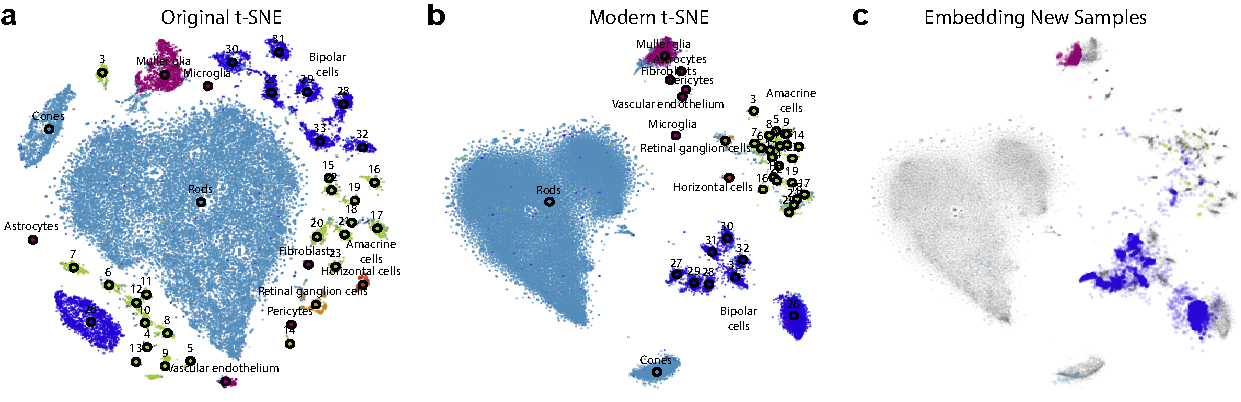
\includegraphics[width=\textwidth]{macosko2015}
  \caption{\label{fig:macosko}
We use \opentsne to generate three t-SNE embeddings and demonstrate recent theoretical advances. The data in \textbf{(a)} and \textbf{(b)} include 44,808 mouse retinal cells that are described with high-dimensional gene-expression profiles from \citet{macosko2015highly}. The data in \textbf{(c)} additionally contains 27,499 expression profiles from mouse retinal cells from \citet{shekhar2016comprehensive}. \textbf{(a)} We construct t-SNE embedding following the parameter choices from the original publication by \citet{maaten2008visualizing}. The visualization shows no preservation of the global organization of clusters, resulting from random initialization and an affinity model focused on preserving local neighborhoods. \textbf{(b)} A modern t-SNE embedding, utilizing the latest theoretical advances and practical recommendations constructed using a multi-scale affinity model, preserving both short-range and long-range interactions between data points and initialized so that the global layout is as meaningful as possible. Unlike in \textbf{(a)}, the green and blue clusters representing different sub-types of amacrine and bipolar cells are now localized to the same regions of the space, indicating a higher level of similarity than to other cell types. The embedding in \textbf{(c)} shows how existing t-SNE reference atlases can be used to place new samples into existing embeddings. The positions of new data points correspond to cell types from the reference atlas.
}
\end{figure*}

Despite its utility, t-SNE has often been criticized for its limited scalability, lack of global organization -- t-SNE identifies well-defined clusters that may be arbitrarily scattered throughout the embedding -- and the absence of theoretically-founded methods to map new data into existing embeddings~\citep{ding2018interpretable,becht2019dimensionality}. Most of these shortcomings have recently been addressed. \citet{linderman2019fast} developed FIt-SNE, an efficient approximation that massively improves the scalability of t-SNE, achieving linear time complexity in the number of samples. \citet{kobak2019art} proposed several techniques to improve global cluster coherence (Fig. \ref{fig:macosko}.b), including estimating similarities with a mixture of Gaussian kernels. In our previous work, we introduced a principled approach for embedding new samples into existing visualizations (Fig.~\ref{fig:macosko}.c and~\citet{policar2021embedding}).

Easy access to efficient implementations almost universally correlates with the widespread adoption of novel computational techniques. Despite the many recent theoretical advancements, popular t-SNE libraries have slowly incorporated them into their implementations.
In \proglang{Python}, the most commonly used implementation of the t-SNE algorithm comes from \pkg{scikit-learn}~\citep{pedregosa2011scikit}, which is nicely integrated with \proglang{Python} data science environment but suffers from poor scalability. Other implementations from the \proglang{R}~\citep{team2013r,krijthe2015rtsne} and \proglang{Julia}~\citep{bezanson2017julia,julia_tsne} programming languages also scale poorly (see Sec.~\ref{s:speed}). \pkg{MulticoreTSNE}~\citep{Ulyanov2016} enjoys better scalability but is likewise limited when applied to larger data sets. Additionally, none of these implementations include recently proposed extensions that can result in more globally consistent embeddings. \pkg{FIt-SNE}~\citep{linderman2019fast} alleviates these problems and provides bindings to both the \proglang{Python} and \proglang{R} programming languages. However, none of the existing t-SNE implementations support adding new samples into existing embeddings. To alleviate all these problems, and to support newly proposed additions to t-SNE algorithms, we here present \opentsne, an open-source \proglang{Python} implementation of the t-SNE algorithm. \opentsne is easy to install and includes precompiled binaries available through popular \proglang{Python} package managers. It provides a familiar API, making it suitable as a drop-in replacement for existing t-SNE implementations.


%% -- Manuscript ---------------------------------------------------------------

%% - In principle "as usual" again.
%% - When using equations (e.g., {equation}, {eqnarray}, {align}, etc.
%%   avoid empty lines before and after the equation (which would signal a new
%%   paragraph.
%% - When describing longer chunks of code that are _not_ meant for execution
%%   (e.g., a function synopsis or list of arguments), the environment {Code}
%%   is recommended. Alternatively, a plain {verbatim} can also be used.
%%   (For executed code see the next section.)

\section{Methods} \label{sec:methods}

We first introduce the relevant notation and briefly review the core t-SNE
algorithm in Sec.~\ref{sec:meth.tsne}. We then address the criticisms of
scalability (Sec.~\ref{sec:meth.approx}), the ability to add new samples to
existing embeddings (Sec.~\ref{sec:meth.transform}), and improvements that
improve the global consistency of resulting embeddings
(Sec.~\ref{sec:meth.global}).

\subsection{$t$-distributed stochastic neighbor embedding} \label{sec:meth.tsne}

$t$-distributed stochastic neighbor embedding (t-SNE) is a non-linear
dimensionality reduction method that to aims to find a low-dimensional embedding
where neighborhoods are preserved. Given a multi-dimensional data set with $N$ data points
$\mathbf{X} = \left \{ \mathbf{x}_1, \mathbf{x}_2, \dots, \mathbf{x}_N \right \}
\in \mathbb{R}^D$, t-SNE
aims to find a low dimensional embedding $\mathbf{Y} = \left \{ \mathbf{y}_1,
\mathbf{y}_2, \dots, \mathbf{y}_N \right\} \in \mathbb{R}^d$ where $d \ll D$,
such that if points $\mathbf{x}_i$ and $\mathbf{x}_j$ are close in the
high-dimensional space, their corresponding embeddings $\mathbf{y}_i$ and
$\mathbf{y}_j$ are also close. Since t-SNE is primarily used as a visualization
tool, $d$ is typically set to two. The similarity between two data points in the
high-dimensional space is defined using the Gaussian kernel
\begin{equation}
p_{j \mid i} = \frac{\exp \left ( -\frac{1}{2} \mathcal{D}(\mathbf{x}_i, \mathbf{x}_j ) / \sigma_i^2 \right )}
{\sum_{k \neq i } \exp \left ( -\frac{1}{2} \mathcal{D}(\mathbf{x}_i, \mathbf{x}_k ) / \sigma_i^2 \right )}, \quad p_{i \mid i} = 0
\label{eq:p_ij}
\end{equation}
where $\mathcal{D}$ is some distance measure. The values $p_{j \mid i}$
are then symmetrized to
\begin{equation}
p_{ij} = \frac{p_{j \mid i} + p_{i \mid j}}{2N}.
\label{eq:symmetrize}
\end{equation}

The bandwidth $\sigma_i$ of each Gaussian kernel is selected such that the perplexity of the distribution matches a user-specified parameter value
\begin{equation}
\text{Perplexity} = 2^{H(P_i)} \notag
\end{equation}
where $H(P_i)$ is the Shannon entropy of $P_i$,
\begin{equation}
H(P_i) = -\sum_i p_{j \mid i} \log_2 (p_{j \mid i}). \notag
\end{equation}
This enables t-SNE to adapt to the varying density of the data in the
multi-dimensional space. The perplexity can be interpreted as the continuous
analogue to the number of nearest neighbors to which the distances will be
preserved. 

The similarity between points $\mathbf{y}_i$ and $\mathbf{y}_j$ in the embedding
space is defined using the $t$-distribution with a single degree of freedom
(Cauchy kernel)
\begin{equation}
q_{ij} = \frac{\left ( 1 + || \mathbf{y}_i - \mathbf{y}_j ||^2 \right )^{-1}}
{\sum_{k \neq l}\left ( 1 + || \mathbf{y}_k - \mathbf{y}_l ||^2 \right )^{-1}},
\quad q_{ii} = 0.
\label{eq:cauchy_kernel}
\end{equation}

We use the Kullback-Leibler (KL) divergence to measure the agreement
between the two distributions $\mathbf{P}$ and $\mathbf{Q}$
\begin{equation}
C = \text{KL}(\mathbf{P} \mid \mid \mathbf{Q}) = \sum_{ij} p_{ij} \log \frac{p_{ij}}{q_{ij}}.
\label{eq:kl_divergence}
\end{equation}
The objective is to find embeddings $\mathbf{Y}$ that minimize the KL divergence. The corresponding gradient takes the form
\begin{equation}
\frac{\partial C}{\partial \mathbf{y}_i} = 4 \sum_{j \neq i} \left ( p_{ij} - q_{ij} \right ) \left ( \mathbf{y}_i - \mathbf{y}_j \right ) w_{ij},
\label{eq:tsne_gradient}
\end{equation}
where $w_{ij} = \left ( 1 + || \mathbf{y}_i - \mathbf{y}_j || ^2 \right )^{-1}$
and represents the unnormalized $q_{ij}$.
Alternatively, this gradient can be rewritten as
\begin{equation}
\frac{\partial C}{\partial \mathbf{y}_i} = 4 \Bigg [
\underbrace{\sum_{j \neq i} p_{ij} q_{ij} Z \left ( \mathbf{y}_i - \mathbf{y}_j \right )}_{\text{attractive forces}}  -
\underbrace{\sum_{j \neq i} q_{ij}^2 Z \left ( \mathbf{y}_i - \mathbf{y}_j \right )}_{\text{repulsive forces}}
\Bigg ], \label{eq:grad_attr_rep}
\end{equation}
where $Z = \sum_{k \neq l}\left ( 1 + || \mathbf{y}_k - \mathbf{y}_l ||^2 \right )^{-1}$. This formulation implies that the t-SNE algorithm can be interpreted as a force-directed layout algorithm, where individual data points act as particles exerting both attractive and repulsive on each other until a state of equilibrium is reached.

Optimization is performed using batch gradient descent using the delta-bar-delta update rule~\citep{jacobs1988increased}. The t-SNE optimization procedure consists of two phases: in the first \textit{early exaggeration} phase, the attractive forces between data points are increased by some factor $\rho$, typically set to $12$, so that points in the embedding can more easily move throughout the space and settle near their respective neighbors. In the second phase of the optimization, the attractive forces are then reverted to their original values with $\rho=1$.

\citet{belkina2019automated} later found that convergence can be sped up by
increasing the learning rate from the standard $\eta=200$ to $\eta=N/12$. As a
side-effect, embeddings converge faster, and the number of iterations can be
lowered from the typical 1000 to 750, decreasing the overall runtime.

\subsection{Efficient approximation schemes} \label{sec:meth.approx}

A direct evaluation of the t-SNE gradients requires $\mathcal{O}(N^2)$ operations, which makes it impractical with large data sets and calls for efficient approximation schemes. The formulation in Equation~\ref{eq:grad_attr_rep} casts the t-SNE gradient as an N-body simulation where data points act as particles exerting attractive and repulsive forces onto one another. Both terms lend themselves to efficient approximations, enabling us to reduce the time complexity of the t-SNE algorithm to $\mathcal{O}(N)$. This allows modern t-SNE implementations to be leveraged for the visualization of data sets containing up to millions of data points.

\subsubsection*{Attractive forces}
\citet{van2014accelerating} observed that evaluating the attractive forces
between all pairs of data points is excessive. In practice, it 
suffices to approximate the attraction forces against a small number of
$k$ nearest neighbors. Using tree-based nearest-neighbor search methods,
\citet{van2014accelerating} reduced the time complexity to $\mathcal{O}(N \log
N)$. \citet{linderman2019fast} noted that embeddings
are visually indistinguishable when using merely \textit{approximate} nearest
neighbors, further reducing time complexity to $\mathcal{O}(N)$.

\subsubsection*{Repulsive forces}
Similarly, the repulsive term can also be approximated, motivated by methods from
particle simulations. \citet{van2014accelerating} proposed an approach based on
N-body simulations and used a space-partitioning Barnes-Hut tree approach to
approximate the interaction between data points. This reduces the time
complexity from $\mathcal{O}(N^2)$ to $\mathcal{O}(N \log N)$. More recently,
\citet{linderman2019fast} proposed an alternative approach, FIt-SNE, based on
non-uniform convolutions, which further reduces the time complexity to
$\mathcal{O}(N)$.

\subsection{Embedding new samples} \label{sec:meth.transform}

The t-SNE algorithm is non-parametric and does not define an explicit mapping from the
high-dimensional space to the embedding space. Embeddings of new data
points need to be found through optimization
schemes~\citep{policar2021embedding}. When adding new data points to an
existing, reference embedding, the reference data points are fixed in place
while new data points are allowed to find their respective positions. The
optimization remains the same as in standard t-SNE with only slight
modifications to $p_{ij}$ and $q_{ij}$
\begin{align}
p_{j \mid i} = \frac{\exp \left ( -\frac{1}{2} \mathcal{D}(\mathbf{x}_i, \mathbf{v}_j) /  \sigma_i^2 \right )}{\sum_{i} \exp \left ( -\frac{1}{2} \mathcal{D}(\mathbf{x}_i, \mathbf{v}_j) / \sigma_i^2 \right )}, \qquad
q_{j \mid i} = \frac{\left ( 1 + || \mathbf{y}_i - \mathbf{w}_j ||^2 \right )^{-1}}{\sum_{i}\left ( 1 + || \mathbf{y}_i - \mathbf{w}_j ||^2 \right )^{-1}}, \notag
\end{align}
\noindent where $\mathbf{V} = \left \{ \mathbf{v}_1, \mathbf{v}_2, \dots,
\mathbf{v}_M \right \} \in \mathbb{R}^D$ where $M$ is the number of samples in
the new data set and $\mathbf{W} = \left \{ \mathbf{w}_1, \mathbf{w}_2, \dots,
\mathbf{w}_M \right \} \in \mathbb{R}^d$. Additionally, we omit the
symmetrization step in Equation~\ref{eq:symmetrize}. Plugging these terms into
Equation~\ref{eq:kl_divergence}, we obtain the following gradient
\begin{equation}
\frac{\partial C}{\partial \mathbf{w}_j} = 2 \sum_i \left ( p_{j \mid i} - q_{j \mid i} \right ) \left ( \mathbf{y}_i - \mathbf{w}_j \right ) \left ( 1 + || \mathbf{y}_i - \mathbf{w}_j || ^2 \right )^{-1}. \notag
\label{eq:gradient}
\end{equation}

Similarly to standard t-SNE, a direct calculation of gradients takes $\mathcal{O}(N \cdot M)$ time, but it is straightforward to adapt the Barnes-Hut and FIt-SNE approximation schemes, reducing the time complexity to $\mathcal{O}(M \log N)$ and $\mathcal{O}(M)$, respectively. Special care must be taken to adjust the learning rate during optimization as the parameter values used during standard optimization lead to highly unstable behaviour. Empirically, we have found that reducing the learning rate to $\eta \sim 0.1$ results in more stable optimization, as discussed in \citet{policar2021embedding}. Moreover, during standard optimization, data points are positioned in the embedding such that an equilibrium between the attractive and repulsive forces is achieved. However, when embedding new data points, the reference embedding remains fixed. Consequently, if a new data point needs to be positioned between existing reference data points, it may not be possible to reach such an equilibrium, as the reference data points cannot adjust to accomodate the new data point. To compensate for the increased repulsive forces, we have found it beneficial to increase the exaggeration factor to $\rho=1.5$ during optimization. The training dynamics of embedding new data points into existing embeddings are yet fully understood and are left to future exploration.


\subsection{Improving the global structure of embeddings} \label{sec:meth.global}

One of t-SNE's long-standing criticisms is that it fails to preserve long-range
distances but instead focuses on capturing the local structure of the data
manifold~\citep{becht2019dimensionality}. Recently, several approaches have been
proposed to improve the global organization of the resulting embeddings.

\citet{kobak2019umap} showed that the initialization of force-directed layout
algorithms, such as t-SNE, UMAP~\citep{2018arXivUMAP}, and
ForceAtlas2~\citep{jacomy2014forceatlas2}, largely dictates the global
consistency of resulting embeddings. When initialized randomly, clusters are
often arbitrarily scattered in the embedding space. However, when using
initialization schemes based on PCA or Laplacian eigenmaps~\citep{belkin2001laplacian}, the clusters identified in the resulting embedding are typically grouped in a globally
coherent manner.

In standard t-SNE, distances between data points are converted to similarities
through the use of Gaussian kernels. The perplexity of these kernels governs the
sizes of the local neighborhoods which are to be preserved. One easy way to
improve the global consistency of resulting embeddings is to increase the sizes
of these neighborhoods. This can be achieved by increasing the perplexity
parameter. However, increasing perplexity often leads to loss in local sturcture
and tends to obscure small clusters. \citet{kobak2019art} instead propose to use
mixtures of Gaussians to preserve better short-range and long-range distances
and, thus, achieve a better trade-off between local and global structure.

Embeddings produced by standard t-SNE often use all available space and separate
clusters by only thin boundaries. When working with large data sets, this often
obscures the global relationships between clusters as all neighboring groups
appear equidistant from one another.  Other dimensionality reduction methods,
such as UMAP and ForceAtlas2, produce embeddings where clusters appear more
compact, and the white space separating the clusters may be interpreted as a
loose measure of distance. Recently, \citet{bohm2020unifying} showed that the
exaggeration factor $\rho$ could be used to produce layouts more similar to UMAP
and ForceAtlas2. By incorporating exaggeration into later phases of the
optimization, t-SNE introduces white space between clusters, which may better
reflect the global relations between clusters.

Standard t-SNE reveals the clustering structure at a single level of resolution.
While the perplexity parameter can be used to control the trade-off between
local and global structure, this can be time-consuming, and small, well-defined
clusters can be missed. Alternatively, \citet{kobak2019heavy} suggest that
varying the degrees of freedom in the $t$-distribution can be used to explore
the clustering structure at different levels of resolution. Modifying
Equation~\ref{eq:cauchy_kernel} to $q_{ij} \propto \left ( 1 + || \mathbf{y}_i -
\mathbf{y}_j ||^2 / \alpha \right )^{-\alpha}$ allows us to use heavier-tailed
distributions to model distances in the embedding space, which acts to highlight
small subgroups in the resulting visualization.


\section{Implementation} \label{sec:implementation}

We introduce \opentsne, a comprehensive \proglang{Python} library that implements the t-SNE algorithm and its numerous recently proposed extensions. \opentsne includes a simple API that allows users to quickly obtain informative t-SNE visualizations and a more flexible API that allows seasoned practitioners to modify all the different aspects of the t-SNE algorithm.

The core t-SNE algorithm comprises three main steps, mirrored in the structure of the \opentsne library:

\begin{enumerate}
\item The t-SNE algorithm requires the specification of an affinity model to describe the similarities between data points $p_{ij}$. Standard t-SNE uses perplexity-based Gaussian kernels with varying bandwidths as specified in Equation~\ref{eq:p_ij}. However, other affinity models can also be used to highlight different aspects of the data or visualize other data modalities. For instance, \citet{kobak2019art} showed that using mixtures of Gaussians often better reveals global cluster organization in the resulting visualization (albeit at some computational cost). Alternatively, a uniform affinity model can produce quantitively similar embeddings to standard t-SNE at a third of the computational cost, making it particularly useful for larger data sets. Unlike the standard affinity model, which uses Gaussian kernels to determine the similarities $p_{ij}$, the uniform affinity model uses a uniform kernel to assign equal similarities to a pre-specified number of nearest neighbors. Visualizing different data modalities, such as graphs, can also be achieved by providing precomputed distance matrices that might consist of, for instance, the shortest paths between nodes. The \code{openTSNE.affinity} module provides a selection of commonly used affinity models but defaults to the standard perplexity-based Gaussian model, as proposed in the original publication. Users can also define custom affinity models by extending the \code{openTSNE.affinity.Affinities} class. The resulting class can then be used as a drop-in replacement for the built-in affinity models.

\item The optimization in t-SNE starts with initial positions for each data point in the embedding space. We can set the initial positions randomly or impose an initial global structure on the embedding. % with, for example, a PCA-based initialization.
The \code{openTSNE.initialization} module provides several possible initialization schemes including random, PCA-based, and Laplacian Eigenmap-based intialization schemes. The user can also specify their own initialization by providing a \code{numpy.ndarray} object. By default, \opentsne opts for PCA-based initialization.

\item In optimizing the embedding, the t-SNE algorithm finds the positions of the points in the embedding space that reflect their corresponding similarities in the affinity model. \opentsne stores the initial positions and affinities in an \code{openTSNE.TSNEEmbedding} object that includes the \code{.optimize} method for embedding optimization that uses either the Barnes-Hut or FIt-SNE approximation scheme. While the FIt-SNE approximation scheme scales linearly with the number of samples, it introduces additional computational overhead, often unnecessary for smaller data sets, resulting in longer overall runtimes than the Barnes-Hut approximation scheme. By default, \opentsne uses an empirically-determined heuristic to choose the fastest algorithm for a given data set based on its number of samples. If the data set contains fewer than 10,000 samples, the Barnes-Hut approximation scheme is selected, otherwise, the FIt-SNE is used.

\end{enumerate}

Once the embedding is constructed and optimized, it is ready to use for any downstream tasks. \code{openTSNE.TSNEEmbedding} objects inherit from \code{numpy.ndarray}, which enables easy manipulation and provides interoperability with the broader \proglang{Python} ecosystem.

Embedding new data points to an existing \code{openTSNE.TSNEEmbedding}
follows the same three general steps as constructing a standard embedding:
\begin{enumerate}
\item Firstly, we must provide an affinity model describing the similarities between each new data point and the data points in the reference embedding. As for the construction of the initial embedding, \opentsne provides several possible affinity models in the \code{openTSNE.affinity} module. Most often, however, we want to utilize the affinity model from the construction of the reference embedding, as this leads to more spatially consistent embeddings. Using an affinity model from reference embedding for the embedding of the new data is the default behavior of \opentsne.


\item Secondly, we must specify the initial positions of the new data points in the embedding space. We can, again, initialize these positions randomly or according to their similarity to the data points in the reference embedding. As before, \opentsne provides several initialization options in the \code{openTSNE.initialization} module, but the user is free to provide their specific initialization.

\item Finally, what remains is a construction of an embedding object, subject to optimization. Because this new embedding relies on an existing reference embedding, we construct a \code{openTSNE.PartialTSNEEmbedding} embedding object, which indicates its dependence on a reference \code{openTSNE.TSNEEmbedding} object. As before, \\
\code{openTSNE.PartialTSNEEmbedding} inherits from \code{numpy.ndarray} and can therefore be easily manipulated. Optimization is, again, performed via the \code{.optimize} method.
\end{enumerate}

\begin{figure*}[htbp]
  \centering
  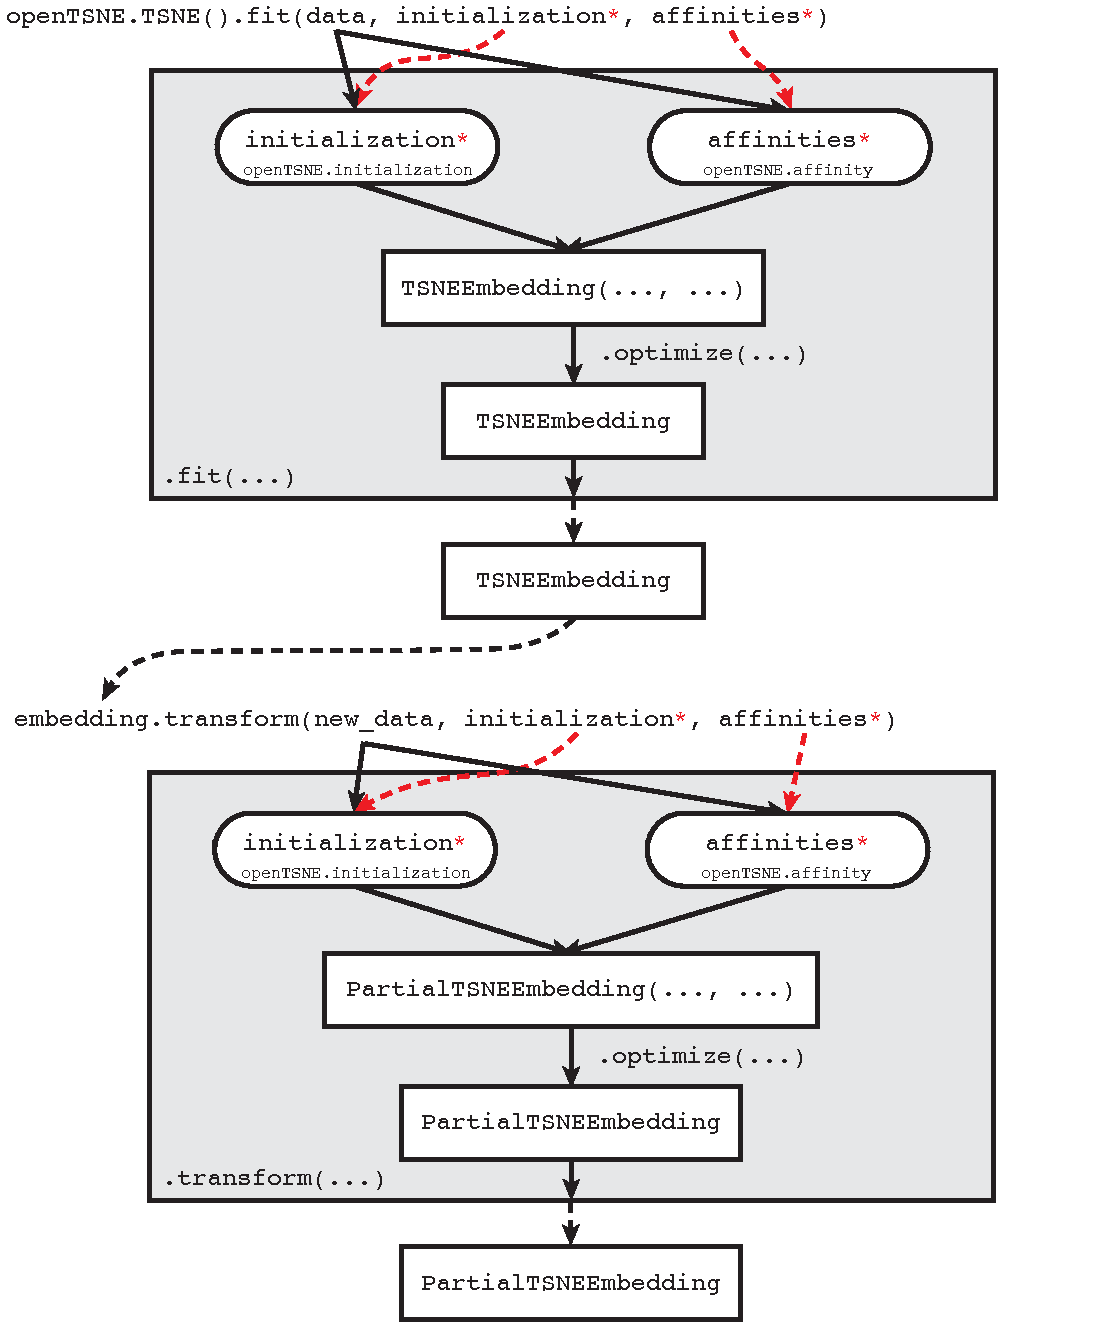
\includegraphics[width=0.9\textwidth]{opentsne-diagram}
  \caption{\label{fig:diagram}
  High-level structure and information flow of the \opentsne library. Solid black lines show the standard parameter flow, while red dashed lines indicate the utility of optional parameters, allowing more refined control over the t-SNE algorithm.
  }
\end{figure*}

Fig.~\ref{fig:diagram} shows the high-level structure and information flow of the \opentsne library. Through different parameters, the user is given complete control over every aspect of the t-SNE data visualization algorithm, from different ways to define affinities to the delicate tuning of optimization parameters. The parametrization of every part of t-SNE allows for rapid experimentation. It enables users to quickly and efficiently inspect their data from numerous angles and at varying levels of resolution.

Most end-users often only need a quick and easy way to create informative visualizations of their data sets. \opentsne provides a high-level API that closely follows the style of \pkg{scikit-learn}~\citep{sklearn_api}, a popular and widely used machine learning toolkit.


\subsection{Example}
\label{sec:iris}

\subsubsection{Installation}

\opentsne is designed to be easy to use and can be installed through either \proglang{Python} Package Index \pkg{PyPI} using package installer \pkg{pip},
\begin{CodeChunk}
\begin{CodeInput}
pip install opentsne
\end{CodeInput}
\end{CodeChunk}
or using package manager \pkg{conda} from the \pkg{conda-forge} repository,
\begin{CodeChunk}
\begin{CodeInput}
conda install -c conda-forge opentsne
\end{CodeInput}
\end{CodeChunk}
\opentsne provides precompiled binaries for all major platforms (Windows, macOS, Linux) for all currently supported \proglang{Python} versions (3.7---3.11). Precompiled binaries are especially convenient for Windows users, as they obviate the need for a \proglang{C}/\proglang{C++} compiler, which is typically not bundled with Windows operating system.

To verify that that \opentsne was installed correctly, users can run \proglang{Python} and try to import the module by:
\begin{CodeChunk}
\begin{CodeInput}
>>> import openTSNE
>>> openTSNE.__version__
1.0.0
\end{CodeInput}
\end{CodeChunk}

\subsubsection{A simple workflow}

We here outline the most straightforward usage of \opentsne on the Iris data set from \citet{anderson1936species}. This small data set profiles 150 iris flowers with four variables (sepal length, sepal width, petal length, petal width) and provides information about their species ({\em Iris Setosa}, {\em Iris Versicolor}, {\em Iris Virginica}). Iris data set comes with \pkg{scikit-learn}:
\begin{CodeChunk}
\begin{CodeInput}
>>> from sklearn import datasets
>>>
>>> iris = datasets.load_iris()
>>> iris.data[:3]
array([[5.1, 3.5, 1.4, 0.2],
       [4.9, 3. , 1.4, 0.2],
       [4.7, 3.2, 1.3, 0.2]])
\end{CodeInput}
\end{CodeChunk}
\pkg{scikit-learn} loads the data set into a \pkg{numpy} array which can directly be used by \opentsne:
\begin{CodeChunk}
\begin{CodeInput}
>>> import openTSNE
>>>
>>> embedding = openTSNE.TSNE().fit(iris.data)
>>> embedding[:3]
TSNEEmbedding([[-0.55581917, 17.56162344],
               [-1.76742536, 20.07763453],
               [-0.58444608, 20.00052495]])
\end{CodeInput}
\end{CodeChunk}
Fig.~\ref{fig:iris} displays the resulting t-SNE visualization. As expected, t-SNE can correctly group samples from the same species. The t-SNE embedding reveals that flowers from {\em Iris Setosa} are markedly different from the other two species. At the same time, flowers from {\em Iris Versicolor} and {\em Virginica} are more similar to one another.
\begin{figure*}[htbp]
  \centering
  \includegraphics[width=0.5\textwidth]{iris}
  \caption{\label{fig:iris}
  A visualization of the constructed t-SNE embedding on the Iris data set. The colors correspond to different species of Iris.
}
\end{figure*}
We can now use the resulting embedding as a reference for new data points. In this simple example, we will duplicate some of the original samples and add them to the embedding.
\begin{CodeChunk}
\begin{CodeInput}
>>> new_data = iris.data[::3]
>>> new_embedding = embedding.transform(new_data)
>>> new_embedding[:3]
PartialTSNEEmbedding([[-0.02637324, 15.69956674],
                      [-2.84200792, 16.15478451],
                      [-2.4594136 , 15.37910876]])
\end{CodeInput}
\end{CodeChunk}
Fig.~\ref{fig:iris-transform} shows the resulting positions of the new data points, overlaid the original, reference embedding. As expected, t-SNE is correctly able to place the new data points to their corresponding groups.
\begin{figure*}[htbp]
  \centering
  \includegraphics[width=0.5\textwidth]{iris-transform}
  \caption{\label{fig:iris-transform}
  A visualization of the original, reference data set (transparent points) overlaid with the new data points (opaque points).
}
\end{figure*}


\subsubsection{Peeking under the hood}

While the above example offers users a quick and easy way to generate informative visualizations, \opentsne allows us to control every step of the t-SNE embedding. To demonstrate this flexibility, we will repeat the exact analysis of the Iris data set as before, this time leveraging the library's more advanced features. We list other practical examples with more complex data sets in Section~\ref{sec:discussion}.

We, again, begin by loading the Iris data set using \pkg{scikit-learn}:
\begin{CodeChunk}
\begin{CodeInput}
>>> from sklearn import datasets
>>>
>>> iris = datasets.load_iris()
>>> iris.data[:3]
array([[5.1, 3.5, 1.4, 0.2],
       [4.9, 3. , 1.4, 0.2],
       [4.7, 3.2, 1.3, 0.2]])
\end{CodeInput}
\end{CodeChunk}
Next, we import the \opentsne library:
\begin{CodeChunk}
\begin{CodeInput}
>>> import openTSNE
\end{CodeInput}
\end{CodeChunk}
We now mirror the three t-SNE steps from the previous section. First, we select an affinity model which describes the similarities between data points:
\begin{CodeChunk}
\begin{CodeInput}
>>> affinities = openTSNE.affinity.PerplexityBasedNN(
...     iris.data, perplexity=30
... )
\end{CodeInput}
\end{CodeChunk}
Next, we determine the initial point positions in the embedding:
\begin{CodeChunk}
\begin{CodeInput}
>>> initialization = openTSNE.initialization.pca(iris.data)
>>> initialization[:3]
array([[-1.30971087e-04,  1.55848907e-05],
       [-1.32435711e-04, -8.63672049e-06],
       [-1.40967409e-04, -7.07276279e-06]])
\end{CodeInput}
\end{CodeChunk}
Finally, using the affinity model and initialization, we can create an embedding object:
\begin{CodeChunk}
\begin{CodeInput}
>>> embedding = openTSNE.TSNEEmbedding(initialization, affinities)
>>> embedding[:3]
TSNEEmbedding([[-1.30971087e-04,  1.55848907e-05],
               [-1.32435711e-04, -8.63672049e-06],
               [-1.40967409e-04, -7.07276279e-06]])
\end{CodeInput}
\end{CodeChunk}
Notice that the embedding object contains the same point coordinates as the initialization: although we have created an \code{openTSNE.TSNEEmbedding} object, we have not yet run any optimization. To optimize the embedding, we have to call the \code{embedding.optimize} method using our desired parameter settings. We use the default parameter settings here, including a shorter early-exaggeration phase, followed by a longer phase with no exaggeration.
\begin{CodeChunk}
\begin{CodeInput}
>>> embedding.optimize(250, exaggeration=12, inplace=True)
>>> embedding.optimize(500, inplace=True)
>>> embedding[:3]
TSNEEmbedding([[-0.55581917, 17.56162344],
               [-1.76742536, 20.07763453],
               [-0.58444608, 20.00052495]])
\end{CodeInput}
\end{CodeChunk}
We can validate that method produces the exact same embedding as before:
\begin{CodeChunk}
\begin{CodeInput}
>>> np.linalg.norm(openTSNE.TSNE().fit(iris.data) - embedding)
0.0
\end{CodeInput}
\end{CodeChunk}
Next, we can add new samples into the embedding,
\begin{CodeChunk}
\begin{CodeInput}
>>> new_embedding = embedding.prepare_partial(iris.data[::3], perplexity=5)
>>> new_embedding.optimize(
...     exaggeration=1.5, n_iter=250, learning_rate=0.1,
...     max_grad_norm=0.25, inplace=True
... )
>>> new_embedding[::3]
PartialTSNEEmbedding([[-0.02637324, 15.69956674],
                      [-2.84200792, 16.15478451],
                      [-2.4594136 , 15.37910876]])
\end{CodeInput}
\end{CodeChunk}
We here use the \code{embedding.prepare_partial} method to determine initial positions for the new data points, then call the \code{new_embedding.optimize} method to run the optimization process. Again, we can validate that this also produces the exact same embedding as before:
\begin{CodeChunk}
\begin{CodeInput}
>>> np.linalg.norm(new_embedding - embedding.transform(iris.data[::3]))
0.0
\end{CodeInput}
\end{CodeChunk}

\section{Case studies} \label{sec:discussion}

We provide three case studies demonstrating the usage of \opentsne in different settings using different combinations of hyperparameters to highlight different aspects of the given data sets.
The first case study highlights how varying the perplexity and resolution parameters can reveal different aspects of the underlying topology of the studied data set.
The second case study demonstrates how \opentsne may be used to create embeddings of massive data sets containing millions of data points and how its flexible API allows the quick and efficient construction of embeddings.
The final case study illustrates how we can use existing t-SNE embeddings to add new samples into the embedding space. This enables us to reuse carefully annotated visualizations for the rapid characterization of new, unseen data points.

\subsection{Uncovering structure in high-dimensional data}

Dimensionality reduction techniques implicitly assume that high-dimensional data lies on a lower-dimensional manifold, which can accurately be captured by a small number of dimensions. However, there is no evidence that every data set can accurately be described using only two dimensions, and any such embedding will inevitably lead to a loss of information. Thus, it is beneficial to examine multiple embeddings, each providing a different perspective on topology and other data characteristics.

\begin{figure*}[htbp]
  \center
  \includegraphics[width=\textwidth]{tasic2018}
  \caption{\label{fig:tasic}
  We use \opentsne to create four different
  visualizations of the \citet{tasic2018shared} data,
  each providing a different perspective into the topology of the data.
  The data set contains 21,874 single-cells originating from the mouse
  neocortex. Cluster annotations and colors are taken from the original
  publication. Warm colors correspond to excitatory neurons, cool colors
  correspond to inhibitory neurons, and gray/brown colors correspond to
  non-neuronal cells. Standard t-SNE \textbf{(a)} emphasizes local
  structure while increasing perplexity \textbf{(b)} results in a more
  meaningful layout of the clusters. We can also combine the two
  perplexities by using a multi-scale kernel affinity model \textbf{(c)}
  and obtain a trade-off between global and local structures.
  Alternatively, we can inspect more fine-grained structures and reveal
  smaller clusters by using a more heavy-tailed kernel \textbf{(d)}.}
\end{figure*}

We illustrate the benefits of creating different t-SNE plots of the same data set by generating four different embeddings of the data on single-cell gene expression in mouse brain~\citep{tasic2018shared}. We generate the embeddings using the following code snippet (shortened for clarity):
\begin{CodeChunk}
\begin{CodeInput}
embedding_a = openTSNE.TSNE(perplexity=30).fit(x)
embedding_b = openTSNE.TSNE(perplexity=500).fit(x)
embedding_c = openTSNE.TSNE(perplexity=[30, 500]).fit(x)
embedding_d = openTSNE.TSNE(perplexity=30, dof=0.6).fit(x)
\end{CodeInput}
\end{CodeChunk}
Fig.~\ref{fig:tasic}.a shows an embedding using default t-SNE parameters. While different clusters of excitatory and inhibitory neurons appear close to one another, all clusters appear equidistant from their neighbors, and the overall relations between groups are not obvious. The embedding in Fig.~\ref{fig:tasic}.b focuses on preserving larger neighborhoods of points, resulting in a more globally consistent layout where relations between clusters become more apparent. Here, it is evident from the increased white space between groups that there is one large class of excitatory neurons and two related classes of inhibitory neurons. Unfortunately, focusing on preserving large neighborhoods leads to the absorption of smaller clusters into larger ones. Alternatively, Fig.~\ref{fig:tasic}.c uses multi-scale similarity kernels that aim to preserve both the global organization of clusters and prevent smaller cluster absorption. We constructed the embedding from Fig.~\ref{fig:tasic}.d with the settings used for Fig.~\ref{fig:tasic}.a, but at a finer level of resolution. The figure demonstrates that some clusters are composed of numerous, smaller subgroups representing different cell subpopulations that are not visible under standard parameter settings.

\subsection{Embedding massive data sets}

When dealing with data containing millions of data points, standard t-SNE embeddings often become unwieldy -- cluster boundaries are blurred, large clusters absorb smaller ones, and relationships between groups become increasingly difficult to interpret. We constructed Fig.~\ref{fig:cao}.a from the data containing expression profiles of over two million single cells captured at different time points in mouse development. The embedding reveals numerous clusters with transitions between time points marked by the color coding, which are difficult to interpret. \citet{kobak2019art} suggest that increasing attractive forces between similar data points controlled via the \textit{exaggeration} parameter leads to more compact clusters and, subsequently, more informative visualizations. For instance, \ref{fig:cao}.b doubles the default exaggeration, which uncovers some of the data's overall structure. Further doubling the exaggeration in \ref{fig:cao}.c allows us to observe that the data is comprised of two main groups of cells and eight somewhat smaller clusters. The visualization also reveals several tiny clusters, possibly corresponding to rare cell types.

\begin{figure*}[htbp]
  \includegraphics[width=\textwidth]{cao2019}
  \caption{\label{fig:cao}
  Increasing the exaggeration parameter leads to compact clusters, highlighting the data's global organization and emphasizing the continuous nature of cell state transitions. The data set from \citet{cao2019single} contains expression profiles from 2,058,652 single cells. The data were collected from mice embryos at different developmental stages daily after 9.5 to 13.5 days. \textbf{(c)} reveals that the data is comprised of two main components -- the neural tube and mesenchymal cells -- as well as several other smaller clusters. The colors indicate developmental progression, where red indicates the least-developed cells and blue indicates the most developed cells. The overall developmental trajectory is most apparent with higher exaggeration levels, showing red cells slowly transitioning into blue cells. Progressively easing the exaggeration factor uncovers finer clusters within the larger groups, as shown in \textbf{(b)} with exaggeration of two and subsequently in \textbf{(a)}, where we show the standard t-SNE with no exaggeration. 32,011 putative doublets are excluded from the visualizations. }
\end{figure*}

Exaggeration can highlight transitions between cell stages in developmental studies. Standard t-SNE often produces embeddings with clearly defined, discrete clusters. We can adjust the level of granularity and resolution of the clusters with several parameters, as shown in Fig.~\ref{fig:tasic}. However, discrete clusters are often undesired in developmental studies where cells' stage is assumed to follow a continuous transition path. To this end, researchers have used other embedding techniques such as UMAP and ForceAtlas2 to better capture the continuity between cell stages. Recently, \citet{bohm2020unifying} showed that embeddings produced by t-SNE with exaggeration values of 4 and $\sim30$ construct embeddings that are markedly similar to UMAP and ForceAtlas2, respectively. For example, in Fig.~\ref{fig:cao}.a, the developmental trajectory between different time points is difficult to observe due to many sprawled out clusters. On the other hand, it is easier to trace the development when we increase the exaggeration factor from $1$ to $2$ to $4$ in Figs.~\ref{fig:cao}.b-c.

We have used the following code to create Figs.~\ref{fig:cao}.a-c and to demonstrate how we can take advantage of the more advanced features of \opentsne to more quickly create meaningful visualizations of massive data sets.

First, we take small subset of data points and create a t-SNE embedding using a high perplexity value to emphasize the high level structure:
\begin{CodeChunk}
\begin{CodeInput}
indices = np.random.permutation(list(range(x.shape[0])))
x_sample, x_rest = x[indices[:25000]], x[indices[25000:]]

init_sample = openTSNE.TSNE(perplexity=500).fit(x_sample)
\end{CodeInput}
\end{CodeChunk}
Next, we will use this embedding to determine the starting positions for the remaining data points:
\begin{CodeChunk}
\begin{CodeInput}
init_rest = init_sample.prepare_partial(x_rest)
\end{CodeInput}
\end{CodeChunk}
Lastly, we merge \code{init_sample} and \code{init_rest} and restore the original ordering to obtain the full initialization:
\begin{CodeChunk}
\begin{CodeInput}
init_full = np.vstack((init_sample, init_rest))[np.argsort(indices)]
\end{CodeInput}
\end{CodeChunk}

Next, we precompute the affinity model. This can take quite a long time and, this way, we can reuse the same affinity model in various different embeddings, without having to repeat the same, costly computation every time:
\begin{CodeChunk}
\begin{CodeInput}
affinities = openTSNE.affinity.PerplexityBasedNN(x, perplexity=30)
\end{CodeInput}
\end{CodeChunk}

Using our precomputed initialization and affinity model, we are now ready to create our \code{TSNEEmbedding} object and optimize the embedding to our liking: 
\begin{CodeChunk}
\begin{CodeInput}
embedding = openTSNE.TSNEEmbedding(init_full, affinities)

embedding_ee = embedding.optimize(n_iter=500, exaggeration=12)
embedding_c = embedding_ee.optimize(n_iter=500, exaggeration=4)
embedding_b = embedding_c.optimize(n_iter=500, exaggeration=2)
embedding_a = embedding_b.optimize(n_iter=500, exaggeration=1)
\end{CodeInput}
\end{CodeChunk}


\subsection{Embedding new samples}

Unlike other popular dimensionality reduction techniques such as principal component analysis or autoencoders, t-SNE is a non-parametric method and does not define an explicit mapping to the embedding space. Therefore, embeddings of new data points need to be found through optimization~\citep{policar2021embedding}. \opentsne is currently the only publicly available library allowing users to add new samples to existing embeddings in a principled manner.

Figs.~\ref{fig:macosko}.b and \ref{fig:macosko}.c demonstrate how we can use a previously labeled single-cell data set and embed cells from a separate experiment into the reference landscape. The reference data from \citet{macosko2015highly} contains gene expression profiles from mouse retinal cells. By embedding the samples from a similar experiment on bipolar retinal cells by \citet{shekhar2016comprehensive}, we can correctly map the bipolar cell clusters onto the reference embedding.

The following snippet shows the code necessary to generate Fig.~\ref{fig:macosko}.

We first construct Fig.~\ref{fig:macosko}.a with the most commonly used parameter values which aims to show that these can lead to poor cluster separation and an overall lack of global consistency:
\begin{CodeChunk}
\begin{CodeInput}
tsne_old = openTSNE.TSNE(
    initialization="random", learning_rate=200, n_iter=750
).fit(x)
\end{CodeInput}
\end{CodeChunk}
We generate the embedding from Fig.~\ref{fig:macosko}.b using parameter values emphasizing the global coherence of the resulting visualization. By default, \opentsne uses PCA-based initialization and automatically determines the optimal learning rate. This allows \opentsne to lower the default number of iterations to 500. To emphasize the global consistency of the resulting embedding, we can also specify multiple perplexity values, resulting in a multiscale affinity model:
\begin{CodeChunk}
\begin{CodeInput}
tsne_multiscale = openTSNE.TSNE(perplexity=[50, 500]).fit(x)
\end{CodeInput}
\end{CodeChunk}

Finally, we can embed new samples into our obtained embedding space:
\begin{CodeChunk}
\begin{CodeInput}
new_embedding = tsne_standard.transform(x_new)
\end{CodeInput}
\end{CodeChunk}

Embedding single cells into existing reference atlases can also be useful for cell-type classification in cases of unknown cell identities. For instance, in Fig.~\ref{fig:transform}, we construct a reference embedding (using the same code snippet as above) using labeled data from \citet{hochgerner2018conserved} containing gene-expression profiles of cells from the mouse brain. The authors assign a type to each cell. We can verify their classification accuracy by visualizing the expression of well-established gene markers for the major cell types. We then embed cells from \citet{harris2018classes} into the constructed cell atlas. In \citet{harris2018classes}, labels are provided only for neuronal cells. We can quickly identify other non-neuronal cell types in the resulting mapping, including oligodendrocytes and astrocytes. We can further use marker genes to validate that the mapping in the reference landscape is correct.

\begin{figure*}[htbp]
  \includegraphics[width=\textwidth]{transform_hochgerner}
  \caption{\label{fig:transform}
  \opentsne supports embedding new samples into an existing reference t-SNE landscape. For the series of visualizations shown in this figure, we first construct a t-SNE embedding for the data from \citet{hochgerner2018conserved} containing 24,185 developing, single cells from the mouse hippocampus. The data contains gene expression in different neurons, supporting glia, and other vascular cells (upper left). Each data point corresponds to a single cell colored according to its inferred cell type as determined in the original publication. We use the same color scheme as in Fig.~\ref{fig:tasic} where warm colors correspond to excitatory neurons, cool colors correspond to inhibitory neurons, and gray/brown colors correspond to non-neuronal cells. We then embed new hippocampal cells collected in a study by \citet{harris2018classes} using the embedding of \citet{hochgerner2018conserved} data as a reference. In their research, \citet{harris2018classes} collected 6,971 single-cells and focused on identifying different types of inhibitory neurons. However, almost half of the collected cells are not neurons and were left uncharacterized. Inspecting the embeddings of these cells in the reference embedding (bottom left) reveals that in addition to inhibitory neurons, the data contains several supporting glial cells and a small population of endothelial cells. We can verify our approach's accuracy by inspecting marker genes for the major cell types in the reference (top row) and embedded samples (bottom row).}
\end{figure*}

The examples presented above demonstrate how to use \opentsne to quickly gain insight into newly-sequenced, single-cell data sets by utilizing existing cell atlases. The approach is general and not limited to single-cell gene expression. One can, in principle, apply it to any tabular data set regardless of the research field or origin of the data.

\section{Discussion} \label{sec:discussion}

\subsection{Versatility}

The ability to use and combine different optimization approaches to construct different embedding spaces is another of \opentsne's core design principles. \citet{kobak2019art} recently provided several recommendations and tricks to obtain better and more meaningful t-SNE visualizations. These include multi-scale similarity kernels, perplexity annealing, and increasing exaggeration when working with massive data sets. \opentsne provides a flexible API to incorporate these improvements in just a few lines of code. Furthermore, \opentsne supports custom affinity models, enabling users to construct t-SNE embeddings on non-tabular relational data: the only requirement imposed by the affinity model is a notion of similarity between data points. Finally, \opentsne's comprehensive callback system can be utilized to monitor and adapt different stages of the optimization phase and has been used to construct visually appealing animations of the t-SNE optimization process.

\subsection{Speed}\label{s:speed}

% General problem statement
One of the t-SNE's common criticisms is limited scalability to large data sets containing, for instance, millions of data points~\citep {becht2019dimensionality}. Slow response times stem from the optimization procedures and their specific implementation in popular open-source libraries. Most implementations of t-SNE have been based on either a direct implementation of the t-SNE algorithm with asymptotic time complexity $\mathcal{O}(N^2)$~\citep{maaten2008visualizing}, or the Barnes-Hut approximation with asymptotic time complexity $\mathcal{O}(N \log N)$~\citep{van2014accelerating}. Recently, however, \citet{linderman2019fast} developed a novel approximation -- FIt-SNE -- which reduces the asymptotic time complexity to $\mathcal {O}(N)$, enabling scaling to large data sets.

% We benchmark Python
Fig.~\ref{fig:benchmarks_py} benchmarks four popular \proglang{Python}~\citep{vanrossum1995python} t-SNE implementations, including \pkg{scikit-learn} (v1.1.2), \pkg{MulticoreTSNE} (v0.1), \pkg{FIt-SNE} (v1.1.0), and \opentsne (v1.0.0). Benchmarks were performed on an Intel(R) Xeon(R) CPU E5-1650 equipped with 128 GB of memory. Benchmarks were run for $1,000$ iterations with the original t-SNE parameters, as some implementations do not allow for their modification. To ensure a realistic benchmarking scenario, we utilize the 10X Genomics 1.3 million mouse brain data set~\citep{cao2019single}, containing 1.3 million single-cell gene-expression profiles. We preprocess the data using the standard single-cell analysis pipeline~\citep{kiselev2019challenges} and extract the top 50 principal components. To generate benchmark data sets of different sample sizes, we subsample the data set five times at each sample size. In total, we test each implementation on 30 different data sets.

\begin{figure*}[ht]
  \centering
  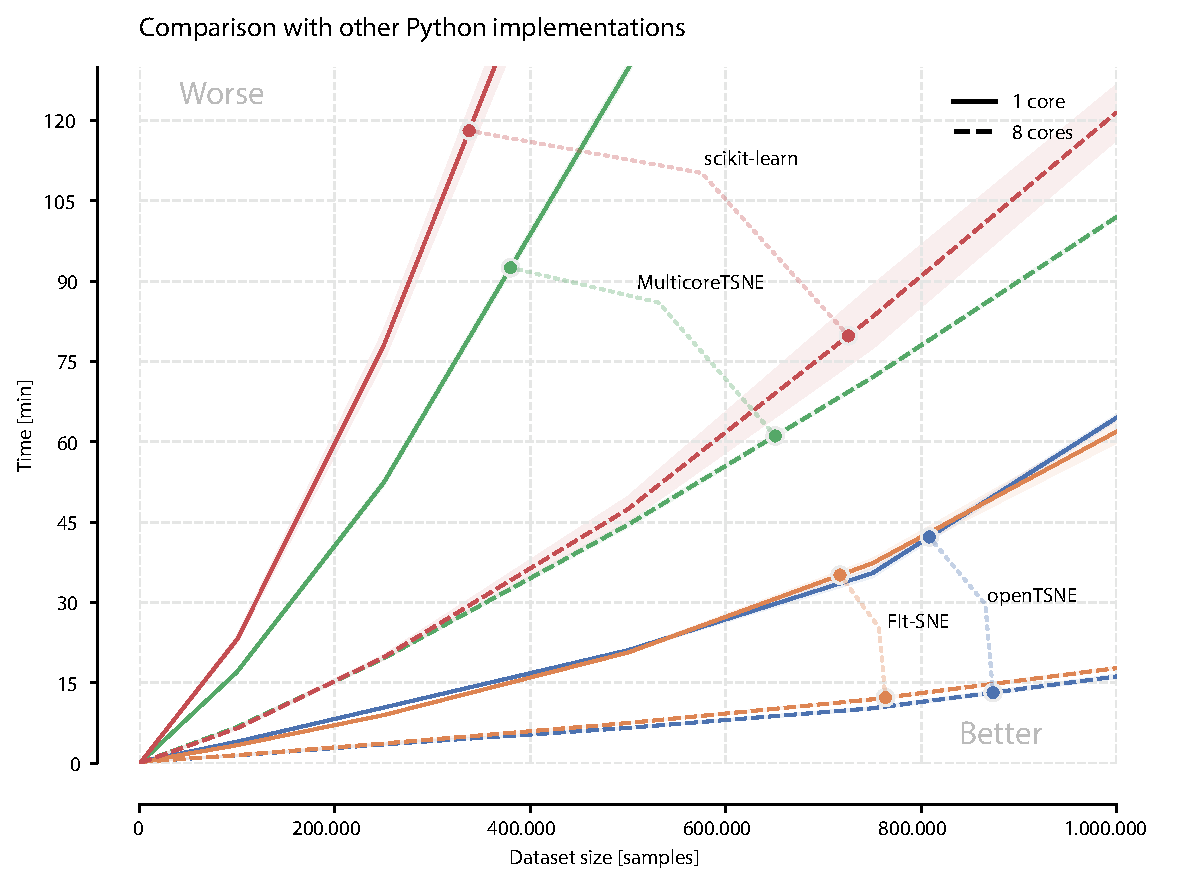
\includegraphics[width=0.75\textwidth]{benchmarks_python-final}
  \caption{\label{fig:benchmarks_py}
  We benchmark \opentsne (v1.0.0) against three popular open-source
  implementations from \pkg{scikit-learn}~\citep{pedregosa2011scikit}
  (v1.1.2), \pkg{MulticoreTSNE}~\citep{Ulyanov2016} (v0.1), and
  \pkg{FIt-SNE}~\citep{linderman2019fast} (v1.1.0). Experiments were run on a
  on an Intel(R) Xeon(R) CPU E5-1650 equipped with 128 GB of memory. Notice
  that \opentsne scales similarly to \pkg{FIt-SNE}, as they both use the
  same interpolation-based approximation scheme, while \pkg{scikit-learn} and
  \pkg{MulticoreTSNE} utilize the Barnes-Hut approximation.
}
\end{figure*}

% Problem with Python
In \proglang{Python}, the most widely-used implementation of t-SNE comes from \pkg{scikit-learn}, which exhibits long runtimes when compared to other \proglang{Python} implementations. \pkg{scikit-learn}, like its \proglang{C++} counterpart -- \pkg{MulticoreTSNE}~\citep{Ulyanov2016} , is based on the Barnes-Hut approximation scheme. However, as shown in Fig.~\ref{fig:benchmarks_py}, \pkg{scikit-learn} exhibits somewhat longer runtimes than \pkg{MulticoreTSNE}. Newer implementations, such as \pkg{FIt-SNE} and \opentsne, implement the FIt-SNE approximation scheme, making them suitable for the visualization of millions of data points. While both libraries implement the same algorithm, \opentsne emphasizes ease of use and extensibility and is primarily written in \proglang{Python}. Despite this, both libraries exhibit similar runtimes, with \opentsne even being marginally faster when utilizing multi-threading, as shown in Fig.~\ref{fig:benchmarks_py}.

Additionally, \opentsne provides a flexible API, allowing the user to split the embedding-construction process into several parts. This modularity enables us to cache and reuse intermediate results, allowing users to experiment with different parameter settings and iterate on their final visualizations. Such functionality is not supported in other t-SNE implementations, which require the user to start from scratch for every embedding, resulting in large amounts of redundant computation.

% Problem with other programming languages
In other programming languages, the selection of fast, open-source implementations of t-SNE is more limited. In \proglang{R}~\citep{team2013r}, the most widely used implementation of t-SNE -- \pkg{Rtsne}~\citep{krijthe2015rtsne} -- is based on the Barnes-Hut approximation, and is closely comparable to \pkg{MulticoreTSNE}. In \proglang{Julia}~\citep{bezanson2017julia}, the most popular implementation -- \pkg{TSne.jl}~\citep{julia_tsne} -- is based on a naive $\mathcal{O}(N^2)$ implementation of the algorithm, which allows it to be used only on smaller data sets containing up to thousands of data points. We benchmark \pkg{Rtsne} (v0.15) and  \pkg{TSne.jl} (v1.3.0) and compare it to \opentsne (v1.0.0). Fig.~\ref{fig:benchmarks_lang} illustrates the scaling of each approximation scheme. Of these implementations, only \opentsne can scale to data sets containing millions of data points in a reasonable amount of time.

\begin{figure*}[ht]
  \centering
  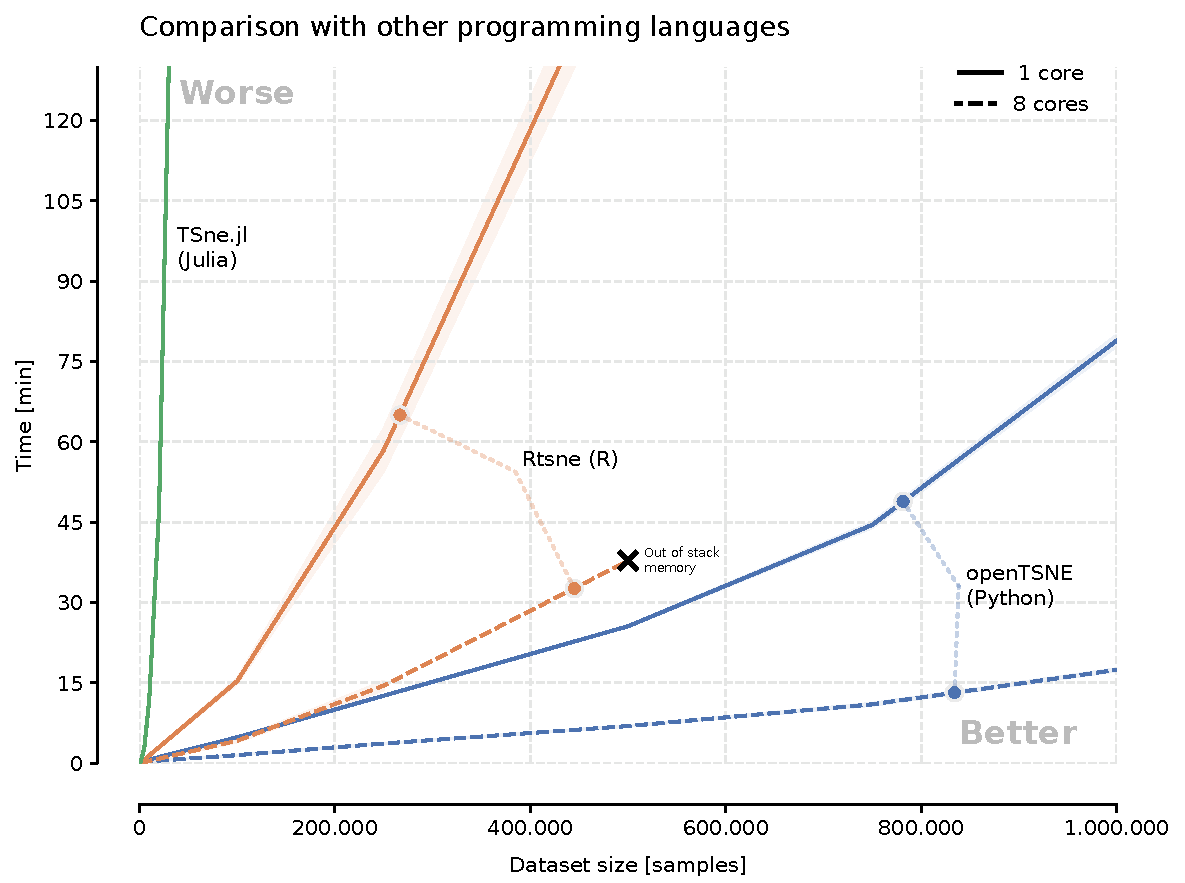
\includegraphics[width=0.75\textwidth]{benchmarks_langs-final}
  %\includegraphics[width=\textwidth]{benchmarks-combined}
  \caption{\label{fig:benchmarks_lang}
  We select the fastest available, open-source implementations of the t-SNE algorithm from the \proglang{Python}, \proglang{R}, and \proglang{Julia} programming languages. We choose \opentsne (v1.0.0) for \proglang{Python}, \pkg{Rtsne}~\citep{krijthe2015rtsne} (v0.15) for \proglang{R}, and \pkg{TSne.jl}~\citep{julia_tsne} (v1.3.0) for \proglang{Julia}. The benchmarks reflect the time complexity of the implemented approximation schemes. For instance, \pkg{TSne.jl} implements a naive $\mathcal{O}(N^2)$ algorithm, making it prohibitively expensive for all but the smallest of data sets. \pkg{Rtsne} scales similarly to \pkg{MulticoreTSNE} in \proglang{Python}, as it implements the $\mathcal{O}(N \log N)$ Barnes-Hut approximation scheme. Interestingly, the multi-threaded implementation version of \pkg{Rtsne} crashes on benchmark data sets containing over 500,000 data points due to a lack of stack memory. We found these crashes to be inconsistent and somewhat random. \opentsne is the only library implementing the more recent FIt-SNE approximation scheme, which makes it suitable for larger data sets. }
\end{figure*}

We note here that the benchmarks in Figs.~\ref{fig:benchmarks_py}~and~\ref{fig:benchmarks_lang} were run for 1,000 iterations to ensure a fair comparison between different implementations. However, it has recently been shown that, using an appropriate learning rate, we can safely reduce the number of iterations to 750~\citep{belkina2019automated}. This means that the actual runtime will be faster than reported in these benchmarks in everyday usage of \opentsne.

\subsection{Ease of use}

Intuitive access and simple installation procedures typically correlate with the widespread adoption of novel computational techniques. While the t-SNE implementation from \pkg{scikit-learn} fits this requirement, its implementation is prohibitively slow for even moderately-sized data sets that span tens of thousands of data records. Other \proglang{C++} implementations such as \pkg{MulticoreTSNE} and \pkg{FIt-SNE} exhibit better scaling in more massive data sets, but the packages do not provide precompiled binaries and require users to compile the software themselves. This problem is critical, for instance, for users of the Windows operating system, where the \proglang{C++} compiler does not come with the system, making the correct configuration of current t-SNE implementations cumbersome.

We designed \opentsne to be accessible to a broader audience. We provide precompiled binaries for all major \proglang{Python} versions on all major platforms, making the installation process as seamless as possible. One can install \opentsne through the \proglang{Python} Package Index (\pkg{PyPI}) or \pkg{conda} from the \pkg{conda-forge} channel, the two most widely adopted \proglang{Python} package managers. \opentsne's high-level interface is inspired by \pkg{scikit-learn}, which is well established in the \proglang{Python} data science ecosystem. \opentsne implements multi-threaded versions of the Barnes-Hut and FIt-SNE approximation schemes, enabling it to be applied to data sets containing millions of data points. Finally, \opentsne is extensible. Its modular design enables researchers to experiment quickly with different parameter settings and easily incorporate custom components into the software. We provide an extended list of features and comparison to other popular t-SNE implementations in Tab.~\ref{tab:features}.

\begin{table}
\begin{center}\small
\newcommand*\rot{\rotatebox{90}}
\renewcommand{\arraystretch}{1.25}

\begin{tabular}{l c c c c|c c}
\toprule
\setlength\tabcolsep{6pt}
& \rot{\pkg{scikit-learn}} & \rot{\pkg{MulticoreTSNE}} & \rot{\pkg{FIt-SNE}} & \rot{\pkg{openTSNE}} & \rot{\pkg{Rtsne}} & \rot{\pkg{Tsne.jl}} \\

\toprule
\textbf{Ease of installation} \\
\pkg{PyPI} package & \checkmark & \checkmark & \checkmark & \checkmark & & \\
\pkg{conda} package & \checkmark & & \checkmark & \checkmark & & \\

\hline
\textbf{Approximation schemes} \\
None ($\mathcal{O}(N^2)$) & & & & & & \checkmark \\
Barnes-Hut ($\mathcal{O}(N \log N)$) & \checkmark & \checkmark & & \checkmark & \checkmark & \\
FIt-SNE ($\mathcal{O}(N)$) & & & \checkmark & \checkmark & & \\

\hline
\textbf{Advanced features and extensions} \\
Extensible affinity models & & & & \checkmark & & \\
Variable degrees of freedom & & & \checkmark & \checkmark & & \\
Variable exaggeration & & & \checkmark & \checkmark & & \\
Globally-consistent initialization & & & \checkmark & \checkmark & & \\
Automatic learning rate & & & \checkmark & \checkmark & & \\
Adding samples to embeddings & & & & \checkmark & & \\
Callback system & & & & \checkmark & & \\
Interactive optimization  & & & & \checkmark & & \\

\hline
\textbf{Project quality}\\
Actively maintained & \checkmark & & & \checkmark & \checkmark & \checkmark \\
Continuous integration & \checkmark & \checkmark & & \checkmark & \checkmark & \checkmark \\
User documentation & \checkmark & & & \checkmark & \checkmark  & \\
End-to-end usage examples & \checkmark & & \checkmark & \checkmark & \checkmark & \checkmark \\
API reference & \checkmark & & & \checkmark & \checkmark &  \\
\bottomrule
\end{tabular}
\end{center}

\caption{\label{tab:features}
  We compare the features of \opentsne~(v1.0.0) to \pkg{scikit-learn}~(v1.0.1),
  \pkg{BHTSNE}~(master), \pkg{MulticoreTSNE}~(v0.1), and
  \pkg{FIt-SNE}~(v1.1.0), as well as the major implementations in \proglang{R}
  and \proglang{Julia}, \pkg{Rtsne}~(v0.15), \pkg{Tsne.jl}~(v1.3.0). Active
  maintenance indicates whether the project has had any meaningful development
  in the past year from the time of writing.
}
\end{table}


\section{Conclusion}

We introduce \opentsne, the most feature-complete, open-source, \proglang{Python} implementation of the widely popular t-SNE visualization algorithm. The library incorporates the latest developments to the t-SNE algorithm and makes them easily accessible through a familiar API. \opentsne implements efficient approximation schemes, making it suitable for visualizing large data sets containing up to millions of data points. Finally, \opentsne is easy to install and comes with precompiled binaries available for all major platforms.

%% -- Optional special unnumbered sections -------------------------------------

\section*{Availability and documentation}

\opentsne is distributed under the BSD-3-Clause License and its source code is
publicly available at \url{https://github.com/pavlin-policar/openTSNE}.
\opentsne can also be installed from \pkg{PyPI} and \pkg{conda-forge}.
End-to-end usage examples, documentation, and API reference are all available at
\url{https://opentsne.readthedocs.io}.

\section*{Reproducibility}

The results in this paper were obtained using \proglang{Python}~3.10.2 with the
\pkg{openTSNE}~v1.0.0 package. All results and figures can be reproduced using
the scripts found in the accompanying GitHub repository
\url{https://github.com/pavlin-policar/opentsne-paper}.
Detailed instructions are provided showing how to reproduce all materials and results shown in this manuscript.

All case studies can easily be reproduced on a consumer-grade laptop computer in minutes using the accompanying scripts. Note, however, that the second case study features a large data set and may require up to several hours to complete.

Scripts are included to reproduce the benchmarks of the different implementations of the t-SNE algorithm. However, please be aware that the full benchmark suite can take several days to complete due to the poor performance of other libraries. A smaller, illustratory benchmark suite is provided, more suitable for consumer-grade laptop computers, demonstrating the runtimes of the different t-SNE implementations. Please note, however, that the scaling advantages of \opentsne are diminished when running on smaller data sets and will not appear as significant as they would otherwise.


\section*{Acknowledgments}

We want to thank Dmitry Kobak for helpful discussions regarding t-SNE and his
contributions to the source code. We would also like to thank George Linderman
for his help with the FIt-SNE algorithm. This work was supported by Slovenian
Research Agency (P2-0209, L2-3170).


%% -- Bibliography -------------------------------------------------------------
%% - References need to be provided in a .bib BibTeX database.
%% - All references should be made with \cite, \citet, \citep, \citealp etc.
%%   (and never hard-coded). See the FAQ for details.
%% - JSS-specific markup (\proglang, \pkg, \code) should be used in the .bib.
%% - Titles in the .bib should be in title case.
%% - DOIs should be included where available.

\bibliography{references}

\newpage

\begin{appendix}

\section{Single-cell RNA-seq Data Preprocessing}

We here describe the preprocessing steps applied to the single-cell RNA-seq data sets used in Fig.~\ref{fig:macosko}~\citep{macosko2015highly}, Fig.~\ref{fig:tasic}~\citep{tasic2018shared}, Fig.~\ref{fig:cao}~\citep{cao2019single}, and Fig.~\ref{fig:transform}~\citep{hochgerner2018conserved}. The standard single-cell preprocessing pipeline consists of gene filtering, gene selection, data normalization, and dimensionality reduction.

First, we discard genes detected fewer than ten times, then select the 3,000 most highly-variable genes following the gene-selection procedure from \citet{kobak2019art}. We then perform counts-per-median library-size normalization followed by log normalization and standardization without zero-centering. Finally, we extract the top 50 principal components, which are then used to construct subsequent t-SNE embeddings. This pipeline is applied to all the aforementioned data sets with the following exceptions, which serve to better illustrate our points:
\begin{itemize}
  \item In \citet{macosko2015highly}, we perform library-size normalization by computing counts-per-million and apply centering during standardization.
  \item In \citet{hochgerner2018conserved}, we select the 1,000 most variable genes.
\end{itemize}

When embedding additional data points into the existing embedding in Figs.~\ref{fig:macosko}.c and \ref{fig:transform}, we follow the procedure from \citet{policar2021embedding}. Therefore, no preprocessing is applied to the data sets from \citet{shekhar2016comprehensive} and \citet{harris2018classes}, and the similarities between the reference data set and the new data set are computed on the raw counts.

\end{appendix}

\end{document}
